% kapitel6.tex
\chapter{Experimentelle Analyse}
\label{cha:analyse}

Die Implementierung des Algorithmus von Kezdy und McGuinness wurde mit dem reinen Planaritätstest von Boyer und Myrvold verglichen.
Um den Fehler durch äußere Einflüsse bei geringer Laufzeit zu minimieren, wurde die Zeit von $100$ gemessen und anschließend gemittelt.
Einerseits wurden beide Algorithmen auf der \emph{Rome-Library}, einer in \cite{BGLT+97} Testmenge von Graphen, ausgeführt.
Die insgesamt $11528$ Graphen bestehen aus $10$ bis $100$ Knoten.
$8249$ sind nicht planar, davon enthalten $7897$ einen \kf-Minor.

Andererseits wurde ein in \OGDF enthaltener Generator genutzt, um zufällige Graphen mit bis zu $10000$ Knoten und variierender Kantenanzahl zu erzeugen.
Um vor allem den Kern des Kezdy-McGuinness Algorithmus, dem Behandeln von \kdd-Minoren, zu Testen, wurden ausschließlich $3$-zusammenhängende Graphen erzeugt.
Dadurch beeinflussen weder Block-Cut Trees noch SPQR-Bäume die Laufzeit.
Außerdem wird kein Zertifikat für den Fall erstellt, dass ein \kf-Minor gefunden wurde.
Ist kein \kf-Minor im Eingabegraph enthalten, liegt immer ein Zertifikat vor, da der Algorithmus die Wagner-Struktur aufbaut.

Getestet wurde auf einem Intel Core i7-9700k mit 3GHz und 32GB RAM.
Als Compiler wurde der GCC 7.3.0 verwendet.

\begin{figure}[H]
  \centering
  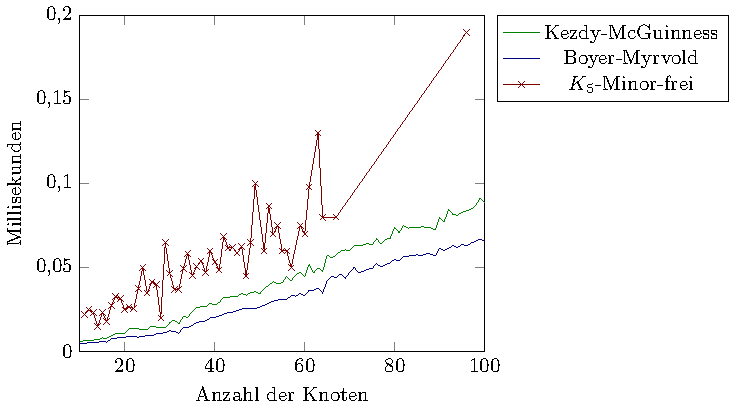
\includegraphics[width=\textwidth,height=\textheight,keepaspectratio]{plots/Benchmarks_Rome.pdf}
  \caption{Benchmark mit den Graphen der Rome Library.}
  \label{fig:Benchmarks-Rome}
\end{figure}

In \Abb \ref{fig:Benchmarks-Rome} ist die Laufzeit in Millisekunden pro Graph zu sehen.
Es fällt auf, dass sich die Laufzeit vom Kezdy-McGuinness-Algorithmus (grün) stark an der des Planaritätstests (blau) orientiert und damit eher linear als quadratisch ist.
Die theoretische Worst-Case-Laufzeit tritt in diesem Anwendungsfall selten auf, da, wie in \Abb \ref{fig:Statistics-Rome} zu sehen, die meisten Graphen entweder planar sind oder einen \kf-Minor enthalten.
Ist ein Graph planar, kann der Algorithmus nach einmaligem Ausführen des Planaritätstests beendet werden, sodass die Laufzeit fast identisch zum reinen Ausführen des Planaritätstests ist.
Der Mehraufwand begründet sich in dem Aufbauen der nötigen Datenstrukturen wie der Wagner-Struktur oder der Kopie des Originalgraphen, die aus $3$-zusammenhängende Komponenten besteht.
Außerdem findet der Planaritätstest oft direkt einen \kf-Minor oder einen \kdd-Minor, der kein \dd-Separator ist, sodass auch in den beiden Fällen der Kezdy-McGuinness-Algorithmus früh terminieren kann.
\Abb \ref{fig:Statistics-Rome} ist zu entnehmen, dass viele Graphen entweder einen \kf-Minor enthalten oder planar und \kf-Minor-frei sind.
Deshalb wurde in \Abb \ref{fig:Benchmarks-Rome} zusätzlich die Laufzeit des Kezdy-McGuinness-Algorithmus (rot) für \kf-Minor-freie Graphen, die nicht planar sind, gemessen.
Da nicht für alle Knotenanzahlen solche Graphen vorliegen, wurden die tatsächlichen Messpunkte markiert.
Hier wird deutlich, dass der Algorithmus deutlich länger läuft, weil der Planaritätstest \dd-Separatoren findet und rekursiv auf die augmentierten Komponenten angewendet wird.
Generell ist in \Abb \ref{fig:Statistics-Rome} aber zu sehen, dass \dd-Separatoren nur in ungefähr $10\%$ der Graphen vorkommen.

\begin{figure}[H]
  \centering
  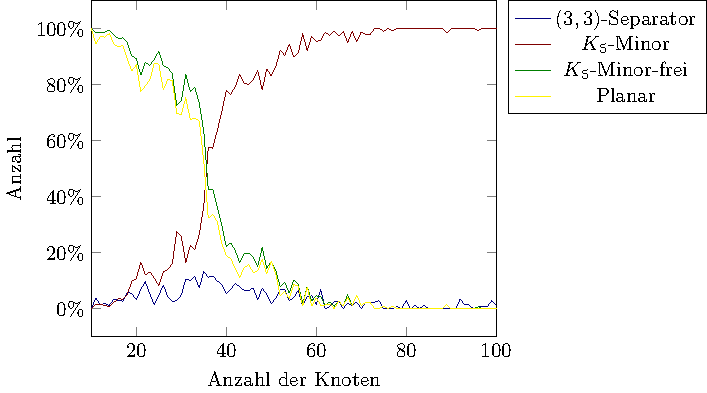
\includegraphics[width=\textwidth,height=\textheight,keepaspectratio]{plots/Statistics_Rome.pdf}
  \caption{Angaben, wie viele Graphen \dd-Separatoren und/oder \kf-Minor enthalten \bzw wie viele planar und/oder \kf-Minor-frei sind.}
  \label{fig:Statistics-Rome}
\end{figure}

\begin{figure}[H]
  \centering
  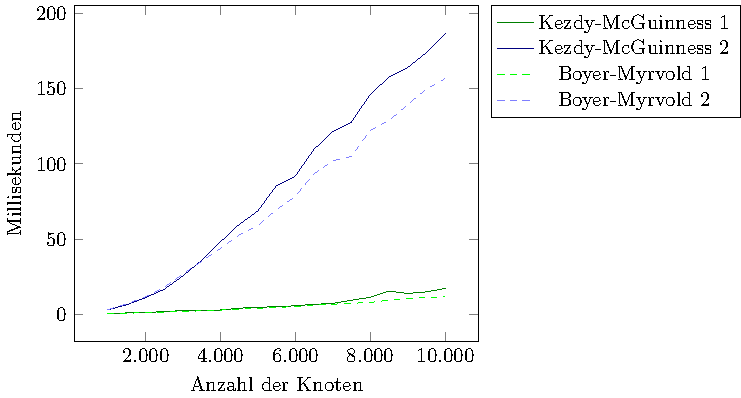
\includegraphics[width=\textwidth,height=\textheight,keepaspectratio]{plots/Benchmarks_Triconnected.pdf}
  \caption{Benchmark $3$-zusammenhängender Graphen mit $n$ Knoten und $2*n$ Kanten (grün) \bzw $10*n$ Kanten.}
  \label{fig:Benchmarks-Triconnected}
\end{figure}

\begin{figure}[H]
  \centering
  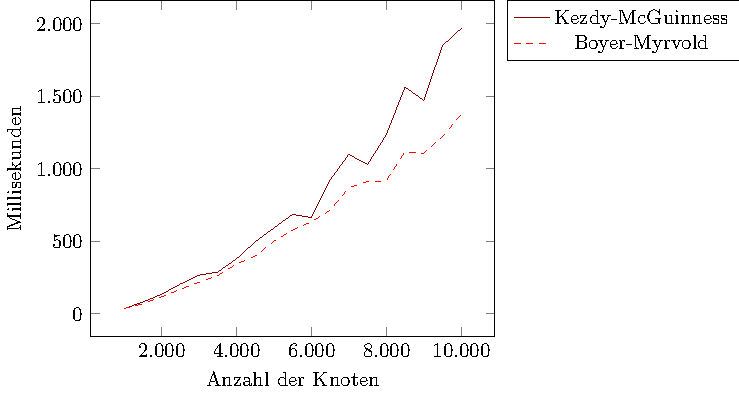
\includegraphics[width=\textwidth,height=\textheight,keepaspectratio]{plots/Benchmarks_TriconnectedVeryDense.pdf}
  \caption{Benchmark $3$-zusammenhängender Graphen mit $n$ Knoten und $f * n$ Kanten für $30 \leq f \leq 100$.}
  \label{fig:Benchmarks-Triconnected-Very-Dense}
\end{figure}

In \Abb \ref{fig:Benchmarks-Triconnected} und \Abb \ref{fig:Benchmarks-Triconnected-Very-Dense} sind die Laufzeiten für größere Graphen zu sehen.
Es wurden für $20$ unterschiedliche Knotengrößen jeweils $25$ Graphen erzeugt und die Zeit über $10$ Iterationen gemittelt.
Die Messungen in \Abb \ref{fig:Benchmarks-Triconnected} decken sich mit denen der Rome-Library.
Die Graphen in \Abb \ref{fig:Benchmarks-Triconnected-Very-Dense} für größere Kantenanzahlen variieren dagegen deutlicher.
Vermutlich wird für die langsameren Instanzen durch den Planaritätstest ein \kdd-Minor gefunden.
Würde er einen \dd-Separator bilden, müsste die Laufzeit deutlich langsamer sein, wie etwa die Messungen für \kf-Minor-freie Graphen in \Abb \ref{fig:Benchmarks-Rome} zeigen.
Allerdings funktioniert der Test, ob der \kdd-Minor ein \dd-Separator ist, über Tiefensuchen, die durch die deutlich höhere Kantenanzahl länger laufen.
Es sei außerdem erwähnt, dass durch die hohe Kantenanzahl immer ein \kf-Minor enthalten ist.

\ \\

Zuletzt wurden in \Abb \ref{fig:Benchmarks-Small} Graphen mit wenigen Knoten und Kanten getestet.
Es wurden nur $10$ Graphen pro Knotenanzahl erzeugt, dafür jedoch in einem kleineren Intervall.
Gemittelt wurde über $100$ Iterationen.
Dadurch, dass nur $10$ Graphen pro Messpunkt getestet wurden, variiert die Laufzeit deutlich stärker.
In \Abb \ref{fig:Statistics-Small} wurde angegeben, wie viele \dd-Separatoren durchschnittlich gefunden wurden.
Es wird deutlich, dass der Kezdy-McGuinness-Algorithmus schneller ist, umso weniger \dd-Separatoren gefunden wurden.
Von den Graphen mit $700$ Knoten enthielten im Schnitt $30\%$ einen \dd-Separator, die Laufzeit lag bei $0,685ms$.
Demgegenüber enthielt keiner der Graphen mit $720$, bis $740$ Knoten einen \dd-Separator.
Die Laufzeit für Graphen mit $740$ Knoten lag beispielsweise bei nur $0,532ms$ und liefen damit ähnlich schnell, wie die kleineren Instanzen mit $580$ Knoten.

\begin{figure}[H]
  \centering
  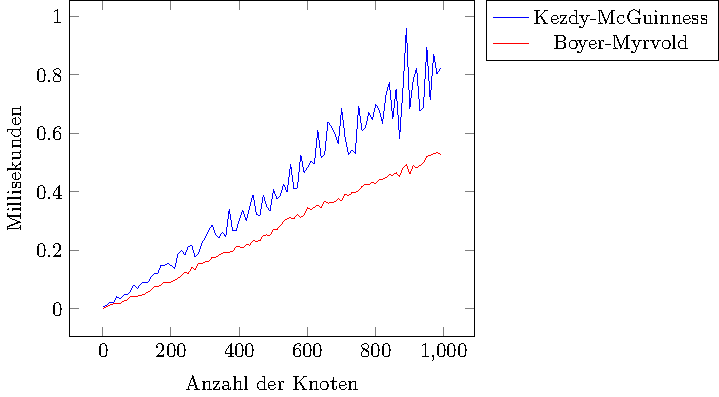
\includegraphics[width=\textwidth,height=\textheight,keepaspectratio]{plots/Benchmarks_Small.pdf}
  \caption{Benchmark für Graphen mit $n$ Knoten und $2*n$ Kanten.}
  \label{fig:Benchmarks-Small}
\end{figure}

\begin{figure}[H]
  \centering
  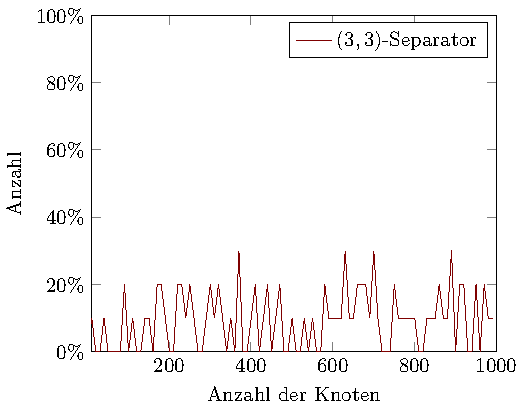
\includegraphics[width=\textwidth,height=\textheight,keepaspectratio]{plots/Statistics_Small.pdf}
  \caption{Angabe, wie viele Graphen mit $n$ Knoten und $2*n$ Kanten einen \dd-Separatoren enthalten.}
  \label{fig:Statistics-Small}
\end{figure}
